\documentclass[conference]{IEEEtran}
\usepackage{cite}
\usepackage{amsmath,amssymb}
\usepackage{booktabs,array}
\usepackage{tikz}
\usepackage{url}
\usetikzlibrary{arrows.meta,positioning}
\newcommand{\RF}{Random Forest}
\newcommand{\SVM}{RBF SVM}
\newcommand{\XGB}{XGBoost}
\newcommand{\smalltable}{\setlength{\tabcolsep}{3.5pt}\renewcommand{\arraystretch}{1.12}\footnotesize}
\title{Stay Upright: Auditable Head-and-Shoulder Posture Classification with Video-Disjoint Evaluation}
\author{\IEEEauthorblockN{Snehal Dixit}
\IEEEauthorblockA{School of Computing Science Engineering and Artificial Intelligence (SCAI)\\
VIT Bhopal University, India\\
snehal.25mip10072@vitbhopal.ac.in}}
\begin{document}
\maketitle
\begin{abstract}
Desktop webcams often show the head and shoulders while the hips remain outside the frame. This paper presents Stay Upright, a posture-awareness pipeline that uses seven visible MediaPipe landmarks to construct a versioned, shoulder-normalized representation and compare Random Forest, radial-basis-function support vector machine, and XGBoost under identical data and split conditions. The contribution is an auditable integration of head-and-shoulder geometry, quality validation that preserves posture-class signals, explicit baseline-label reconciliation, and a shared offline/live feature extractor. A single-volunteer pilot supplies eight protocol-labeled videos and 1,930 accepted frames. Model selection uses chronological development blocks with a two-second gap; evaluation holds out four complete videos containing 968 frames. Random Forest, SVM, and XGBoost achieve macro F1 scores of 0.9835, 0.9510, and 0.9886, respectively. A historical quality audit identifies 421 slouch frames incorrectly removed by upright-assuming geometry checks. An exploratory feature ablation shows that expanded planar features improve discrimination, while inferred depth does not consistently help. A local loopback application supports the validation-selected RF refit, while a browser-only demonstration exposes the three frozen models with checked inference parity. These results establish a reproducible personal-use feasibility study; they do not establish performance on unseen participants or clinical posture validity.
\end{abstract}
\begin{IEEEkeywords}
sitting posture, MediaPipe, head-and-shoulder geometry, Random Forest, support vector machine, XGBoost, video holdout, reproducibility
\end{IEEEkeywords}

\section{Introduction}
Desktop webcams commonly show the face and shoulders while the hips and legs remain outside the image. Requiring reliable hip coordinates can reject usable frames or introduce reliance on extrapolated landmarks. A posture-awareness application must therefore state its observation boundary and avoid treating head movement as a direct measurement of spinal alignment.

MediaPipe provides cross-platform perception \cite{mediapipe}, and BlazePose estimates 33 landmarks \cite{blazepose}. Neither component determines posture labels or an appropriate evaluation protocol. Randomly distributing nearby frames across training and testing can produce optimistic estimates. Recording-level separation and a distinction between personal-use and cross-person evaluation are therefore essential.

Stay Upright extends an existing browser monitor based on two geometric rules into a controlled four-class comparison. The classes are Correct, Slouch, Lean Left, and Lean Right; they denote instructed head-and-shoulder gestures, with left and right defined anatomically. The investigation asks: \emph{How do three conventional classifiers behave under a common observable-landmark representation, a common video-disjoint test, and a preserved rule baseline?} The available evidence is a single-person pilot, and the paper retains that scope throughout.

\subsection{Research Contributions}
The contribution is a tested integration of sensing, preprocessing, evaluation, and deployment. The classifiers themselves are established methods. Four aspects distinguish the implemented study:

\textbf{Observable-region feature design:} seven required visible head/shoulder landmarks produce 21 normalized descriptors without inspecting unseen hips or legs. The retained legacy features support comparison with the original monitor, while signed asymmetry preserves lateral information.

\textbf{Class-retention auditing:} a traceable quality-policy comparison identifies 421 Slouch frames removed by upright-assuming geometry checks. The revised gate restores these observations without reducing the landmark-confidence threshold. This quantifies a preprocessing failure that classifier accuracy alone would conceal.

\textbf{Compatible controlled evaluation:} RF, SVM, and XGBoost use identical rows, video-disjoint testing, and equal candidate budgets. Three-state rules are evaluated against collapsed ML predictions; the four-state directional extension and post hoc ablations are identified separately.

\textbf{Verified browser deployment:} a matching feature contract and readable classifier implementations let users switch among the frozen models while comparing one camera frame. All 5,790 checked browser predictions match Python, linking the scored research artifacts to the deployed demonstration.

These contributions establish engineering feasibility in a single-participant pilot. They do not assert a new learning algorithm, priority over all prior implementations, or validated performance on unseen people.

\section{Related Work and Research Position}
Lee, Choi, and Kim \cite{weightedrf} already classify sitting postures from frontal facial and shoulder features using weighted Random Forest, including lateral lean. Thus, neither a frontal webcam nor face/shoulder features alone constitute the novelty of this project. The distinction here is a specific seven-landmark normalized representation coupled to explicit quality-filter auditing, baseline compatibility, and checked equivalence between Python evaluation and browser deployment.

ML-2SN combines skeletal spatial and temporal streams and addresses lower-body occlusion and action boundaries \cite{ml2sn}. Stay Upright evaluates static geometry and contributes no temporal model. SitPose uses Kinect depth sensing, ensemble learning, and 36 participants \cite{sitpose}; its sensor and evaluation population differ from this webcam pilot.

MultiPosture provides MediaPipe coordinates from 13 participants with upper/lower-body labels \cite{multiposture}. It was assessed but excluded because its trunk labels, coordinate reference, and available joints do not match this feature contract. Equating forward trunk lean with the prompted Slouch gesture without verification would change the task.

RF \cite{rf}, SVM \cite{svm}, and XGBoost \cite{xgb} are established classifier families. This study compares them within one sensing pipeline. Evaluation should approximate the intended use case \cite{saeb}; another recording of the same person does not establish cross-person performance. Table~\ref{tab:position} positions the study without ranking incompatible benchmark scores.

\begin{table}[t]
\caption{Research position relative to representative prior work}
\label{tab:position}\centering\smalltable
\begin{tabular}{p{.23\columnwidth}p{.32\columnwidth}p{.36\columnwidth}}
\toprule Work & Input/approach & Relationship to this study\\\midrule
Lee \emph{et al.} \cite{weightedrf} & Frontal face/shoulder features; weighted RF & Establishes prior use of this observable body region\\
ML-2SN \cite{ml2sn} & Skeletal spatial/temporal streams & Models temporal behavior; present study uses static features\\
SitPose \cite{sitpose} & Kinect depth; ensemble learning & Different sensor and broader participant evaluation\\
MultiPosture \cite{multiposture} & Upper/lower-body joint coordinates & Different labels and feature contract\\
Stay Upright & Seven visible landmarks; common RF/SVM/XGB pipeline & Audited quality gate, reconciled rules, video-disjoint personal pilot\\\bottomrule
\end{tabular}
\end{table}

\section{Proposed Method}
\subsection{Pipeline and Observation Boundary}
Fig.~\ref{fig:pipeline} separates the research path from the live application. Original videos supply the observations; the recording protocol supplies labels; MediaPipe supplies estimated landmarks; and the classifiers operate on the same feature columns. Models are not trained from generated feature values or rule-generated ground truth. Raw video is retained locally for the recording experiment. The optional local application sends landmarks to a loopback Python server; the hosted demonstration computes both features and model predictions inside the browser without transmitting camera observations.

\begin{figure}[t]\centering
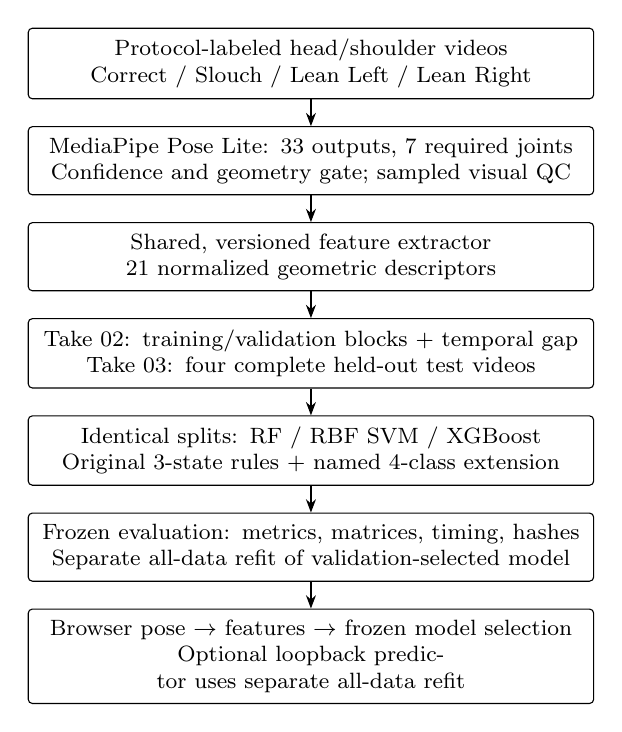
\begin{tikzpicture}[node distance=3.4mm, every node/.style={font=\footnotesize}, box/.style={draw,rounded corners=1.5pt,align=center,text width=6.9cm,inner sep=4pt}, >={Stealth}]
\node[box] (video) {Protocol-labeled head/shoulder videos\\Correct / Slouch / Lean Left / Lean Right};
\node[box,below=of video] (pose) {MediaPipe Pose Lite: 33 outputs, 7 required joints\\Confidence and geometry gate; sampled visual QC};
\node[box,below=of pose] (features) {Shared, versioned feature extractor\\21 normalized geometric descriptors};
\node[box,below=of features] (split) {Take 02: training/validation blocks + temporal gap\\Take 03: four complete held-out test videos};
\node[box,below=of split] (models) {Identical splits: RF / RBF SVM / XGBoost\\Original 3-state rules + named 4-class extension};
\node[box,below=of models] (reports) {Frozen evaluation: metrics, matrices, timing, hashes\\Separate all-data refit of validation-selected model};
\node[box,below=of reports] (live) {Browser pose $\rightarrow$ features $\rightarrow$ frozen model selection\\Optional loopback predictor uses separate all-data refit};
\foreach \a/\b in {video/pose,pose/features,features/split,split/models,models/reports,reports/live} \draw[->] (\a)--(\b);
\end{tikzpicture}
\caption{The implemented pipeline. All scored classifiers use the same test rows. The live refit is kept separate from the frozen evaluation.}
\label{fig:pipeline}\end{figure}

The required indices are $\{0,2,5,7,8,11,12\}$: nose, two eye landmarks, two ears, and two shoulders. The 33-landmark interface is retained, but remaining joints are not inspected for feature calculation or quality acceptance. MediaPipe's normalized image coordinates, rather than metric world coordinates, are used. Its $z$ output is an inferred depth proxy \cite{poseguide}; physical distance and spinal curvature are not recovered.

\subsection{Normalization and Feature Construction}
For image width $W$ and height $H$, let $a=W/H$ and map an image landmark to $p_i=(ax_i,y_i,az_i)$. Let $d$ be planar Euclidean distance, $n$ the nose, $s_l,s_r$ the shoulders, $e_l,e_r$ the ears, $s_m=(s_l+s_r)/2$, and $e_m=(e_l+e_r)/2$. The normalizer is
\begin{equation}
w_s=d(s_l,s_r).
\end{equation}
Distances, coordinate offsets, and relative depth proxies are divided by $w_s$. The normalized quantities reduce sensitivity to uniform body-image scale and translation; they do not guarantee invariance to camera viewpoint, perspective, or landmark estimation errors.

The legacy monitor uses a planar facial triangle on each side, containing eye, ear, and nose. Its incenter is
\begin{equation}
I(A,B,C)=\frac{d(B,C)A+d(A,C)B+d(A,B)C}{d(B,C)+d(A,C)+d(A,B)}.
\end{equation}
Let $D_l=d(I_l,s_l)$, $D_r=d(I_r,s_r)$, and $w_0=d(s_l,s_r)$, calculated in the original normalized $(x,y)$ coordinates for exact rule compatibility. Three retained descriptors are
\begin{equation}
f_1=\frac{10|D_l-D_r|}{w_0},\quad f_2=\frac{D_l+D_r}{w_0},\quad A_s=\frac{D_l-D_r}{w_0}.
\end{equation}
These three deliberately preserve the legacy coordinate convention; the other descriptors use aspect-corrected coordinates. In particular, $f_1$ alone removes the sign needed to represent lateral direction, whereas $A_s$ preserves it.

For a top/bottom point pair, a signed vertical angle is defined as
\begin{equation}
\theta(t,b)=\operatorname{atan2}(t_x-b_x,b_y-t_y),
\end{equation}
reported in degrees. It produces ear-midpoint/shoulder-midpoint inclination and nose/ear-midpoint tilt. The shoulder angle follows $\operatorname{atan2}(s_{r,y}-s_{l,y},s_{l,x}-s_{r,x})$. These are geometric proxies, rather than clinically calibrated neck or torso angles. Table~\ref{tab:features} accounts for all 21 dimensions.

\begin{table}[t]\caption{Feature groups and exact dimensionality}\label{tab:features}\centering\smalltable
\begin{tabular}{p{.21\columnwidth}cp{.64\columnwidth}}
\toprule Group & $N$ & Descriptors\\\midrule
Legacy geometry & 3 & $f_1$, $f_2$, signed facial asymmetry $A_s$\\
Planar ratios & 8 & Nose--shoulder-midpoint; each ear--ipsilateral shoulder; nose--each shoulder; eye-midpoint--shoulder-midpoint; ear width; eye width\\
Signed angles & 3 & Ear/shoulder inclination, head tilt, shoulder angle\\
Planar offsets & 4 & Shoulder height difference; nose vertical and lateral offsets; ear-midpoint vertical offset\\
Depth proxies & 3 & Nose and ear-midpoint depth relative to shoulders; bilateral face/shoulder depth asymmetry\\\midrule
Total & 21 & Seven required landmarks; no hip or leg coordinates\\\bottomrule
\end{tabular}\end{table}

\subsection{Quality Validation and Review}
Every required landmark must have finite coordinates, lie inside the image, and satisfy visibility and available presence scores of at least 0.65. Frames are also rejected for degenerate facial triangles, a planar shoulder span below $0.1a$, or nose--shoulder-midpoint distance exceeding three shoulder widths. Crucially, the gate does not require the nose to lie above the shoulders or impose a minimum nose/shoulder separation. A deep prompted forward gesture can violate those upright assumptions while still providing usable landmarks.

The extraction records rejected frames separately. Sampled skeleton overlays support review, and a review gate requires explicit recording and sampled-frame decisions before producing a clean CSV. Any rejected sampled overlay quarantines its whole recording. In this pilot, an assistant inspected 207 overlays and 24 raw overview images, with decisions and reviewer identity recorded; all eight videos were accepted. This is sampled assistant review, not exhaustive human assessment or expert ground truth. The historical gate correction and the exploratory analysis are disclosed separately from the primary classifier comparison.

\subsection{Models and Rule Compatibility}
The comparison uses RF, RBF SVM, and XGBoost on identical features and row IDs. RF uses 200 trees with balanced class weights and searches maximum depth in $\{\mathrm{None},12\}$. SVM standardizes features within a training-only pipeline and searches $C\in\{1,10\}$ with an RBF kernel and scale-based $\gamma$. XGBoost uses 300 estimators, learning rate 0.05, row and column subsampling 0.8, histogram trees, and a four-class objective; depth is searched in $\{3,6\}$. Each family receives two validation candidates. Stochastic tree models use seed 42 and one worker. Equal candidate counts control search size, not execution time or model capacity.

The exact original fixed-default rule is preserved:
\begin{equation}
\hat y_r=\begin{cases}
\mathrm{Slouch},&f_2-1.352<-0.12,\\
\mathrm{Lean},&|f_1-0.031|>0.55,\\
\mathrm{Correct},&\text{otherwise}.
\end{cases}
\end{equation}
Its precedence is unchanged. Because the rule merges lateral directions, the fair comparison collapses both ML lean classes into Lean and reports three-state metrics. A separately named directional extension uses $A_s<0$ for Lean Left and the opposite sign for Lean Right after the original Lean decision. It is not presented as the unchanged original baseline. Upright calibration is supported in the interactive rule mode, but the recorded baseline uses fixed defaults; no labeled test frames were used for calibration.

\section{Experimental Design}
\subsection{Collection and Data Provenance}
One volunteer, denoted S01, explicitly agreed to webcam recording. Two complete takes per class were recorded with only the head and shoulders required in view. Completed takes carry identifiers 02 and 03; an earlier partial recording was preserved but excluded from the manifest. Clips are approximately 60 seconds, encoded at $640\times480$, with the first and last five seconds excluded from the stable analysis interval. The extractor samples at a target 5 Hz and restarts the VIDEO-mode pose tracker for each clip. The resulting accepted dataset contains 1,930 observations (Table~\ref{tab:counts}). Labels come from the prompted action, not classifier output. Slouch denotes the prompted forward/rounded upper-body gesture and is not a measured spinal diagnosis.

\begin{table}[t]\caption{Recorded pilot dataset and frozen test support}\label{tab:counts}\centering\smalltable
\begin{tabular}{lrrr}\toprule Protocol class & Take 02 & Take 03 & Total\\\midrule
Correct & 236 & 242 & 478\\
Slouch & 242 & 242 & 484\\
Lean Left & 242 & 242 & 484\\
Lean Right & 242 & 242 & 484\\\midrule
Total & 962 & 968 & 1,930\\\bottomrule
\end{tabular}\end{table}

Records retain participant ID, video path, frame index, timestamp, feature version, and pose-asset checksum. Original-video, manifest, cleaned-data, and review checksums provide an audit trail. The feature contract is \texttt{posture-head-shoulders-v2}; the revised quality policy is \texttt{head-shoulders-quality-v3}. Python 3.11.9, MediaPipe 0.10.35, OpenCV 4.14.0, scikit-learn 1.9.1, and XGBoost 3.2.0 were used. The workstation has an Intel Core 7 240H processor and 15.7 GiB reported memory, running Windows. This records the measured environment rather than a standardized hardware benchmark.

\subsection{Selection, Test Separation, and Deployment Refit}
Take 02 is the development set, and every take-03 recording is reserved for testing. Within each development video, the chronological boundary is placed at 70\% of its accepted timestamp span. Training frames end more than one second before the boundary; validation frames begin more than one second after it. Across the four videos, this gives 664 tuning-training frames, 262 validation frames, and 36 gap frames. The gap reduces immediate temporal adjacency but does not make within-video samples independent.

Hyperparameters are selected using validation macro F1 only. A model family is also selected on that criterion; ties follow the deterministic RF/SVM/XGBoost listing order. All chosen configurations are then fitted on the complete 962-frame development set, including the tuning gap, and scored on exactly the same 968 test frames. The split and model-selection decisions are saved before test evaluation.

RF and SVM tie at validation macro F1 0.9807; RF is therefore chosen for the separate personal-use refit. The frozen scored models remain saved. A \emph{separate} RF artifact is refitted on all 1,930 frames for personal live use. Since that refit includes the former test set, the reported test scores describe the frozen take-02 models, not the all-data refit. The hosted comparison uses the frozen models, so its model choices correspond to the scored artifacts. The implementation also supports subject-level holdout and LOSO for future multi-participant data, but those procedures were not run on S01 as evidence of cross-person performance.

\subsection{Metrics and Exploratory Analyses}
Accuracy and class-wise precision/recall/F1 are calculated from the frozen predictions. Macro F1 gives each of the four classes equal weight:
\begin{equation}
F_{1,\mathrm{macro}}=\frac{1}{4}\sum_{c=1}^4\frac{2P_cR_c}{P_c+R_c},
\end{equation}
with a zero contribution for undefined class terms. Reported training time measures the development refit, excluding candidate search. Timing follows a warm-up prediction, then measures both an amortized test batch and median individual predictions for the first 100 test rows. These times include the classifier and SVM scaler, but exclude pose inference, feature extraction, HTTP, rendering, and webcam acquisition.

Two additional analyses were conducted for this manuscript after the primary experiment. A historical audit compares the retained rows of the original and revised extraction artifacts, verifying matching video, manifest, pose-model, sampling-rate, and confidence settings. An exploratory ablation compares the two legacy features, their three-feature signed extension, the 18 features excluding depth proxies, and the full 21 features. Every ablation reuses the frozen split and the same two-candidate validation budget. Because the existing test videos are reused, these analyses are post hoc diagnostics rather than fresh confirmatory experiments; they do not reselect the deployed model.

\section{Results}
\subsection{Four-Class Classifier Comparison}
Table~\ref{tab:performance} reports the primary result. XGBoost has the highest held-out-video accuracy (98.86\%) and macro F1 (0.9886), followed by RF (98.35\%, 0.9835) and SVM (95.14\%, 0.9510). XGBoost's numerical lead over RF is approximately 0.52 percentage points of accuracy, representing five fewer errors. This does not establish a statistically reliable ordering across participants. RF remains the selected refit because its selection preceded testing; the comparison demonstration permits switching among all three frozen models.

\begin{table*}[t]\caption{Primary four-class results on the same 968 take-03 frames (single-person pilot)}\label{tab:performance}\centering\smalltable
\begin{tabular}{lrrrrrrrr}\toprule Model & \shortstack{Accuracy\\(\%)} & \shortstack{Macro\\precision} & \shortstack{Macro\\recall} & \shortstack{Macro\\F1} & \shortstack{Validation\\F1} & \shortstack{Fit\\(s)} & \shortstack{Batch\\(ms/frame)} & \shortstack{Single-frame\\median (ms)}\\\midrule
RF & 98.35 & 0.9845 & 0.9835 & 0.9835 & 0.9807 & 0.287 & 0.0107 & 7.624\\
RBF SVM & 95.14 & 0.9593 & 0.9514 & 0.9510 & 0.9807 & 0.004 & 0.0037 & 0.217\\
XGBoost & 98.86 & 0.9891 & 0.9886 & 0.9886 & 0.9494 & 0.240 & 0.0050 & 0.231\\\bottomrule
\end{tabular}\end{table*}

All three models classify every held-out Slouch, Lean Left, and Lean Right frame correctly in this particular dataset. Their errors occur in Correct: 16 of 242 frames for RF, 47 for SVM, and 11 for XGBoost, all predicted as Slouch. Thus, the practical error mode is false slouch feedback rather than lateral confusion. Correct recall is 0.9339, 0.8058, and 0.9545 for RF, SVM, and XGBoost, respectively. Fig.~\ref{fig:confusion} gives the complete four-class matrices and makes the class imbalance in errors visible.

\begin{figure*}[t]\centering
\newcommand{\cmatrix}[5]{\begin{minipage}{.31\textwidth}\centering\footnotesize\textbf{#1}\\[2pt]\begin{tabular}{c|rrrr}&C&S&L&R\\\hline C&#2&#3&0&0\\S&0&242&0&0\\L&0&0&242&0\\R&0&0&0&242\end{tabular}\\[3pt]Accuracy #4\%; macro F1 #5\end{minipage}}
\cmatrix{RF}{226}{16}{98.35}{0.9835}\hfill
\cmatrix{RBF SVM}{195}{47}{95.14}{0.9510}\hfill
\cmatrix{XGBoost}{231}{11}{98.86}{0.9886}
\caption{Frozen test confusion matrices: rows are actual and columns predicted. C = Correct, S = Slouch, L = Lean Left, R = Lean Right. Each actual class contains 242 frames.}
\label{fig:confusion}\end{figure*}

\subsection{Rule Baseline and Label Reconciliation}
The original three-state rules achieve 97.62\% accuracy and macro F1 0.9756 on the collapsed labels (Table~\ref{tab:baseline}). Under that same label space, RF and XGBoost achieve macro F1 0.9779 and 0.9848, while SVM drops to 0.9346. Therefore, the observations do not support the blanket statement that every ML model outperforms the rules. The small RF gain over the rules is descriptive evidence within this pilot only. The separately named four-class directional rule extension obtains macro F1 0.9762; its result is not substituted for the original rule baseline.

\begin{table}[t]\caption{Fair three-state comparison after collapsing both lean directions}\label{tab:baseline}\centering\smalltable
\begin{tabular}{lrr}\toprule Method & Accuracy (\%) & Three-state macro F1\\\midrule
Original fixed-default rules & 97.62 & 0.9756\\
RF, collapsed predictions & 98.35 & 0.9779\\
RBF SVM, collapsed predictions & 95.14 & 0.9346\\
XGBoost, collapsed predictions & 98.86 & 0.9848\\\bottomrule
\end{tabular}\end{table}

\subsection{Quality-Gate Audit}
The historical extraction accepted 1,509 frames, including only 63 Slouch frames. The revised policy accepted 1,930 frames, including 484 Slouch frames, while retaining the same 478 Correct and 484 frames per lateral class. All formerly accepted row IDs are present in the revised data. Thus, the upright-assuming checks removed 421 of the 484 potentially retained Slouch observations (86.98\%). Correcting those assumptions restored the class without lowering the 0.65 confidence threshold.

This is a concrete example of preprocessing erasing a target-class signal: head descent or a short nose/shoulder separation is precisely part of the recorded gesture. It demonstrates the need to audit rejection rates by protocol class. It does not prove that every newly accepted landmark is anatomically accurate; sampled overlays and independent human review remain important.

\subsection{Exploratory Feature Ablation}
Table~\ref{tab:ablation} reports macro F1 for each representation. The two-feature representation yields 0.6575 for RF, 0.6428 for SVM, and 0.7100 for XGBoost. Adding signed asymmetry improves lateral information and raises those scores to 0.8467, 0.8729, and 0.8418. Expanding the planar representation produces further gains in this split.

Depth proxies do not consistently improve performance. The 18-feature SVM reaches 1.0000 on these already-used test videos, compared with 0.9510 for the full 21-feature SVM. RF changes only slightly, and XGBoost is unchanged to the displayed precision. The 18-feature SVM result is an exploratory outcome, not a new claim of perfect generalization. Its validation score (0.9689) was lower than the full SVM's (0.9807), illustrating why test-driven feature or model reselection would bias the reported performance. The deployed RF configuration is unchanged.

\begin{table}[t]\caption{Exploratory ablation: macro F1 on the reused frozen test videos}\label{tab:ablation}\centering\smalltable
\begin{tabular}{lrrrr}\toprule Representation & $N$ & RF & SVM & XGB\\\midrule
Legacy $f_1,f_2$ & 2 & 0.6575 & 0.6428 & 0.7100\\
Legacy + signed asymmetry & 3 & 0.8467 & 0.8729 & 0.8418\\
All except depth proxies & 18 & 0.9845 & 1.0000 & 0.9886\\
Full representation & 21 & 0.9835 & 0.9510 & 0.9886\\\bottomrule
\end{tabular}\end{table}

\subsection{Runtime and Live Integration}
Median model-only individual inference takes 7.624 ms for RF, 0.217 ms for SVM, and 0.231 ms for XGBoost. The RF batch time is much lower per frame because the overhead is amortized. These are distinct measurements and should not be converted into a claimed application frame rate. End-to-end browser latency and fresh webcam accuracy were not measured.

The hosted demonstration bundles the same Pose Lite asset and Tasks Vision 0.10.35 JavaScript/WebAssembly runtime alongside the three frozen take-02 classifiers. A readable JavaScript feature implementation preserves the Python feature order and quality checks. RF inference averages leaf probabilities, multiclass RBF SVM evaluates six pairwise decisions after the saved scaling transform, and XGBoost accumulates class-specific tree margins. The selected model controls the main posture feedback while a comparison panel shows all three predictions for the same frame. The interface also supports mirrored preview, optional landmark drawing, fullscreen presentation, session timing, posture-transition counters, and access to the manuscript and code explanation. Mirroring changes display only; lateral labels remain anatomical. Camera frames and landmarks remain on the device. ML mode disables rule calibration because the trained representation uses absolute normalized features.

A parity check compares the JavaScript features and predictions with Python on all 1,930 recorded rows. All 5,790 classifier labels agree; the maximum absolute feature difference is $5.69\times10^{-14}$. This verifies implementation equivalence on the recorded samples, not numerically identical pose tracking across runtimes or accuracy on fresh webcam observations. Invalid tracking clears feedback, and camera stop releases the media tracks. Thirteen Python tests and browser controller checks cover geometry, hidden-lower-body independence, review gates, splits, model switching, invalid tracking, calibration and camera lifecycle. The separate loopback Python predictor and all-data RF refit remain available; they are distinct from the hosted frozen-model demonstration.

\section{Discussion, Limitations, and Reproducibility}
The engineering lesson is that sensing boundaries and preprocessing must match the classification task. Seven required joints make the observable region explicit, while retention audits expose filters favoring upright geometry. Baseline compatibility is equally important: three-state rules require collapsed ML labels or an explicitly named directional extension for a meaningful comparison.

The dataset contains one person, eight prompted clips, and one recording session. Test frames are correlated observations from four videos, not independent participants. Tuning blocks share conditions despite their gap. Subject variability, population confidence intervals, statistical significance, and cross-person ranking are not estimable. High scores may reflect distinct instructed gestures and stable conditions; cross-day, environmental, viewpoint, and natural-use robustness were not measured.

The Slouch class varies in gesture severity and is not certified by an ergonomics professional. Only sampled assistant review was completed; institutional ethics approval or exemption was not documented in the project record. The pilot should therefore be interpreted as personal-use engineering feasibility, not a validated human-subject ergonomic study. Identifiable recording frames are excluded from the manuscript figures. The application makes no claim to diagnose spinal conditions or demonstrate health improvement.

Code, feature order, split row IDs, parameters, versions, hashes, frozen models/predictions, matrices, and review receipts are retained. Primary results are in \texttt{results/pilot\_S01}; diagnostics are in \texttt{results/paper\_analysis\_S01}. A public demonstration is available at \url{https://posture-detection-plum.vercel.app}. A public release of the research dataset and training artifacts is not claimed. Raw videos remain local, and checksums establish artifact traceability rather than clinical label validity.

Future work requires human-reviewed multi-participant data, the applicable institutional research determination, cross-day recordings, and whole-participant evaluation using the existing LOSO/holdout tooling. The feature ablation should be fixed before fresh testing. End-to-end timing, natural-use false feedback, and participant-calibrated rule comparisons are also needed.

\section{Conclusion}
Stay Upright implements a traceable head-and-shoulder posture pipeline from recording through local live inference. Its incremental contribution combines a seven-landmark normalized representation, quality checks that preserve class-related geometry, shared train/live feature computation, and transparent evaluation of conventional classifiers against compatible rules. The one-person video holdout produces macro F1 scores of 0.9835 for RF, 0.9510 for SVM, and 0.9886 for XGBoost; validation selects RF for the separate all-data refit, while the browser comparison uses the frozen evaluated models. The quality audit exposes a large Slouch-retention failure, and the exploratory ablation cautions against assuming that inferred depth always helps. These results support a reproducible feasibility prototype and define the evidence needed for a future multi-participant study.

\begin{thebibliography}{00}
\bibitem{mediapipe} C. Lugaresi \emph{et al.}, ``MediaPipe: A framework for building perception pipelines,'' arXiv:1906.08172, 2019. [Online]. Available: \url{https://arxiv.org/abs/1906.08172}
\bibitem{blazepose} V. Bazarevsky, I. Grishchenko, K. Raveendran, T. Zhu, F. Zhang, and M. Grundmann, ``BlazePose: On-device real-time body pose tracking,'' arXiv:2006.10204, 2020. [Online]. Available: \url{https://arxiv.org/abs/2006.10204}
\bibitem{weightedrf} J. Lee, H. Choi, and J. Kim, ``Classification algorithm for sitting postures using weighted random forest,'' \emph{IET Image Processing}, vol. 19, no. 1, Art. no. e70126, 2025, doi: 10.1049/ipr2.70126.
\bibitem{ml2sn} K. Jia, C. Cheng, G. Zhang, Y. Yang, G. Huang, and P. Wang, ``ML-2SN: A hybrid two-stream system for sitting posture detection,'' in \emph{Proc. British Machine Vision Conf.}, 2024. [Online]. Available: \url{https://bmva-archive.org.uk/bmvc/2024/papers/Paper_510/paper.pdf}
\bibitem{sitpose} H. Jin, X. He, L. Wang, Y. Zhu, W. Jiang, and X. Zhou, ``SitPose: Real-time detection of sitting posture and sedentary behavior using ensemble learning with depth sensor,'' arXiv:2412.12216, 2024. [Online]. Available: \url{https://arxiv.org/abs/2412.12216}
\bibitem{multiposture} D. Carneros Prado, L. Caba\~nero G\'omez, J. Fontecha, R. Herv\'as, I. Gonz\'alez D\'iaz, and E. Johnson, ``MultiPosture: A dataset of body joints keypoints extracted using MediaPipe for multi-task sitting posture recognition with upper and lower body labels,'' Zenodo, 2024, doi: 10.5281/zenodo.14230872.
\bibitem{rf} L. Breiman, ``Random forests,'' \emph{Machine Learning}, vol. 45, pp. 5--32, 2001, doi: 10.1023/A:1010933404324.
\bibitem{svm} C. Cortes and V. Vapnik, ``Support-vector networks,'' \emph{Machine Learning}, vol. 20, pp. 273--297, 1995, doi: 10.1007/BF00994018.
\bibitem{xgb} T. Chen and C. Guestrin, ``XGBoost: A scalable tree boosting system,'' arXiv:1603.02754, 2016. [Online]. Available: \url{https://arxiv.org/abs/1603.02754}
\bibitem{saeb} S. Saeb, L. Lonini, A. Jayaraman, D. C. Mohr, and K. P. Kording, ``The need to approximate the use-case in clinical machine learning,'' \emph{GigaScience}, vol. 6, no. 5, pp. 1--9, 2017, doi: 10.1093/gigascience/gix019.
\bibitem{poseguide} Google, ``Pose landmark detection guide for Python,'' MediaPipe documentation. Accessed: Oct. 7, 2026. [Online]. Available: \url{https://developers.google.com/edge/mediapipe/solutions/vision/pose_landmarker/python}
\end{thebibliography}
\end{document}
